\chapter{Server-side PTAM Architecture}
\label{Chapter3}

In this chapter, we implement a prototype system based on the reference implementation of PTAM \cite{Reference12}. The prototype integrates the five visualization methods in section \ref{VisualizationMethods}. It provides realtime MR video with no requirement for any GPS or gyrocompass devices.

%------------------------------------------------------------------------------

\section{System Architecture}

The prototype can use either a Sony VAIO (appendix \ref{AppendixVAIO}) or an Apple iPhone (appendix \ref{AppendixiPhone}) as the mobile device. We base our program on the PTAM reference implementation source code \cite{Reference16} to get the position and orientation of the camera attached to the mobile device. However, this implementation cannot run on neither mobile devices because it requires a dualcore CPU to be able to run smoothly. In order to add computation power to the prototype system, we connect a MacBook Pro (appendix \ref{AppendixMacBook}) as a PTAM server to the mobile device via wireless network, and the PTAM part of the program is set aside on the PTAM server (figure \ref{fig:PrototypeArchitecture}).

For the sake of quick setup time, the mobile device and the PTAM server are connected directly using ad hoc mode, which means that an additional wireless hub is not needed. This setup also has another advantage that the data transmission is very quick: the ``ping'' time is only about 1 ms. If a hub is used, the ``ping'' time may sometimes go up to 100 ms.

\begin{table}[tb]
	\begin{center}
		\caption{System configuration}
		\label{tb:SystemConfiguration}
		\begin{tabular}{|c|c|c|}
			\hline
			Configuration          & VAIO--MacBook Pro & iPhone--MacBook Pro                      \\
			\hline
			Operating system       & Windows XP SP2    & iPhone OS 2.2, Mac OS X 10.5.6 (Leopard) \\
			Wireless network speed & 11 Mbps           & 54 Mbps                                  \\
			\hline
		\end{tabular}
	\end{center}
\end{table}

On theory the network interfaces on both VAIO and MacBook Pro are able to work at 54 Mbps, but for some reason of Microsoft Windows SP2 they can only work at 11 Mbps (table \ref{tb:SystemConfiguration}). This is an unexpected problem which lowers the speed, and consequently the accuracy and stability of the prototype system. They can be connected via LAN cable for faster 100 Mbps speed, but since the VAIO will be wired to another bulky device, wiring for network is not desirable because the mobility of the VAIO is totally lost.

%------------------------------------------------------------------------------

\section{Server-side PTAM}

We modify the original PTAM source code so that the ``video source'' is remotely located on the mobile device, not on the server where the PTAM process actually runs. We learn a little from Erlang language \cite{Reference17} of how to write concurrent, high-performance systems. Right after the Transmission Control Protocol (TCP) connection between the mobile device and the PTAM server is established:

\begin{itemize}
	\item The mobile device continuously feeds frames captured from its camera to the PTAM server.
	\item The PTAM server continuously feeds position and orientation of the mobile camera to the mobile device.
\end{itemize}

As the above explanation suggests, we use ``push'' style data passing instead of ``pull'', one side actively sends data to the other side without having to wait for the request for the data from the other side. In other words we use the mailbox design pattern instead of the RPC (Remote Procedure Call) design pattern, which is slower and requires synchronizing the call and the result (figure \ref{fig:RPCMailbox}).

\begin{figure}[htbp]
	\centering
	\includegraphics{./Figures/rpc_mailbox.png}
	\rule{35em}{0.5pt}
	\caption[RPC vs. Mailbox]{RPC (above) vs. Mailbox (below)}
	\label{fig:RPCMailbox}
\end{figure}

There are two essential threads in the PTAM process: tracking and mapping threads. The tracking thread tracks feature points in the frames received from the mobile camera, and the mapping thread builds 3D maps of these points. Because the tracking thread only need grayscale frames, instead of sending all the three RGB color channels of each frame, the mobile device only needs to send the brightness Y = 0.3*R + 0.59*G + 0.11*B. There are several optimizations to further improve the frame rate sent to the PTAM server:

\begin{itemize}
	\item Send G color channel instead of Y, because G affects Y the most as in the above common equation. This does not affect PTAM. This optimization enormously improves the frame rate because we can omit the pixel-wise calculation of the brightness estimation.
	\item Losslessly compress G color channel using the standard library ``zlib''. The compression rate is about 50\%. But we should use compression with care because it may take more time to compress and uncompress than to send uncompressed images.
\end{itemize}

\begin{table}[tb]
	\begin{center}
		\caption{Frame rates of various conditions between the VAIO and the MacBook Pro (see table \ref{tb:SystemConfiguration})}
		\label{tb:FrameRates}
		\begin{tabular}{|c|c|c|r|}
			\hline
			Size (only G color channel) & Compressed & With PTAM processing & Frame-per-second \\
			\hline
			320 x 240 & NO         & NO                   &  8.01 \\
			320 x 240 & YES        & NO                   & 10.67 \\
			640 x 480 & NO         & NO                   &  1.97 \\
			640 x 480 & YES        & NO                   &  3.03 \\
			320 x 240 & NO         & YES                  &  6.57 \\
			320 x 240 & YES        & YES                  &  6.23 \\
			640 x 480 & NO         & YES                  &  1.84 \\
			640 x 480 & YES        & YES                  &  1.69 \\
			\hline
		\end{tabular}
	\end{center}
\end{table}

However, as table \ref{tb:FrameRates} suggests, we should use 320 x 240 frame size with uncompressed G color channel for the VAIO--Macbook Pro configuration. Bigger frame size allows PTAM to find more feature points, but the following drawbacks pop up:

\begin{itemize}
	\item Data for each frame gets bigger. This increases data transmission time for each frame.
	\item The PTAM server must consume computation power on the bigger frame. This decreases the result frame rate.
\end{itemize}

When the image size is enlarged from 320 x 240 to 640 x 480, the frame rate drops about 4 times, and the prototype no longer works smoothly as required in \ref{VisualizationRequirements}.

Color channels of the camera frames are not saved separately, but in the format BGR for each pixel. Hence to extract the G color channel from each frame we cannot do it in one pass by calling ``memcpy'' the whole channel, we must do a pixel-wise loop through all the pixels of each frame. This processing does consume some computation power of the mobile device. Consequently, it may be faster to send all the BGR values to the PTAM server in one pass, rather than extracting the G color channel. Because the computation power of the mobile device is far weaker than that of the server, we should make the right decision: which frame size should we take and when should we extract the G color channel and/or compress the data?

The answer is that we should not make any optimization as long as the wireless network is not saturated the data for each frame. The tracking thread of the PTAM server can work well with about 7 FPS, hence for example in case of 11 Mbps network, the data size threshold for each frame is 11 x 1024 x 1024 / 8 / 7 = 205970 Bytes. We should not apply any optimization if the data for each frame is less than this threshold:

\begin{itemize}
	\item 320 x 240 x 1 color channel = 76800 ($<$ 205970)
	\item 324 x 240 x 3 color channels = 230400 ($>$ 205970)
	\item 640 x 480 x 1 color channel = 307200 ($>$ 205970)
\end{itemize}

Color channel extraction is lighter than data compression, hence we can conclude that for the VAIO the frame rate is the best if we use 320 x 240 and G color channel extraction for 11 Mbps network. For the iPhone (see table \ref{tb:SystemConfiguration}), we can do similar calculation. However, due to its hardware limitation the frame is fixed at 304 x 400 x BGRA (4 channels). The similar calculation suggests that we should not apply any optimization.

On the mobile device, there are pre-registered positions and orientations of surveillance cameras as described in section \ref{SceneModel}. Having the position and orientation of itself tracked and fed by the PTAM server, the mobile device can overlay the visual aids on the screen precisely.

%------------------------------------------------------------------------------

\section{PTAM Map Initializing and Scene Model Pre-registering}
\label{MapInitializing}

PTAM continuously builds and maintains a 3D map by adding stable feature points and removing unstable ones taken from the frames (figure \ref{fig:Map}).

\begin{figure}[htbp]
	\centering
	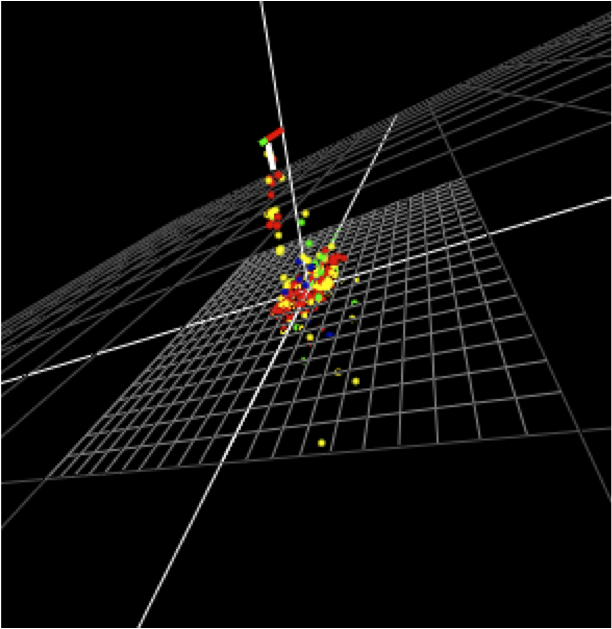
\includegraphics{./Primitives/map.png}
	\rule{35em}{0.5pt}
	\caption[A PTAM map]{A PTAM map. Color of the feature points indicates stability levels: red $>$ yellow $>$ green $>$ blue $>$ light yellow.}
	\label{fig:Map}
\end{figure}

The problem is the 3D scene model (section \ref{SceneModel}) must be in match with this map. We assume that the scene is unchanged. Thus we have the following workflow:

\begin{enumerate}
	\item Initialization and registration phase: Let PTAM build the map. Manually translate and rotate the scene model to match the map (or vice versa), then save the translation and rotation parameters.
	\item Usage phase: On the next program startup, as long as we can make sure that the map is not different from the map used to save the parameters, we can use the parameters to translate and rotate the scene model to match the map.
\end{enumerate}

The reference implementation of PTAM initializes the map on every startup by taking two keyframes which form a stereo pair. As a result, there are two considerable approaches to initiate the map-model matching:

\begin{itemize}
	\item Control the two keyframes. This approach is easy because we simply take two images before-hand, then feed them to the PTAM server on every startup. We prepare two images of the scene as we can have reliable feature points in the map. The PTAM process allows the user at startup to stand at a slightly different position from the ones where we took the two images (figure \ref{fig:2KeyFrames}).
	\item In the initialization and registration phase, serialize the map to string and save the string to disk, then on booting up the PTAM process just skip the map initialization, load the map from disk, deserialize and feed it directly to the PTAM process. We can prebuild a large fine-grained map beforehand, thus the system becomes very robust. With this approch, a user can stand at many different positions and orientations at start up, as long as the position is inside the prebuilt map.
\end{itemize}

The second approach is in general more powerful than the first one, but if the scene changes too much then it may be less powerful because parts of the prebuilt map will become invalid and cause noise or heavy load to PTAM. The first approach always works given a small static scene where the two images were taken, because the map can be updated dynamically by PTAM.

With the first approach, because of the reference implementation of PTAM requirement to make the map initialization stable, actually we must take about 5-10 images and feed them to PTAM, with the first and the last one act as the two keyframe (figure \ref{fig:2KeyFrames}). The video retrieving part and feature point processing part of PTAM run in two separate threads, as a result slightly different maps may be initialized each time the PTAM process starts. Because the tracking and mapping parts run in two separate threads, to make sure that the PTAM process always initialize the same map, we must feed each frame for an enough amount time, so that the two threads have enough time to process and communicate with each other to build the same initial map on every startup. This amount of time is about one second for the MacBook Pro we are using.

\begin{figure}[htbp]
	\centering
	\includegraphics[width=14cm]{./Figures/2keyframes.png}
	\rule{35em}{0.5pt}
	\caption[Feeding frame to PTAM to initialize map]{Feeding frame to PTAM to initialize map}
	\label{fig:2KeyFrames}
\end{figure}

%------------------------------------------------------------------------------

\section{Fusion of GPS and Gyrocompass Devices}

The PTAM based camera registration as described in the previous section is quite robust and it has the advantage that it requires only a single camera as for hardware. However, the PTAM based approach does not always work well. For example it may not work when the images taken in real scene is too different from the images used to build the initial PTAM map because of lighting condition changes. We need other sensor support to enhance the applicability of our prototype system. That are GPS and gyrocompass devices as in figure \ref{fig:VAIOGPSGyro}.

\begin{figure}[htbp]
	\centering
	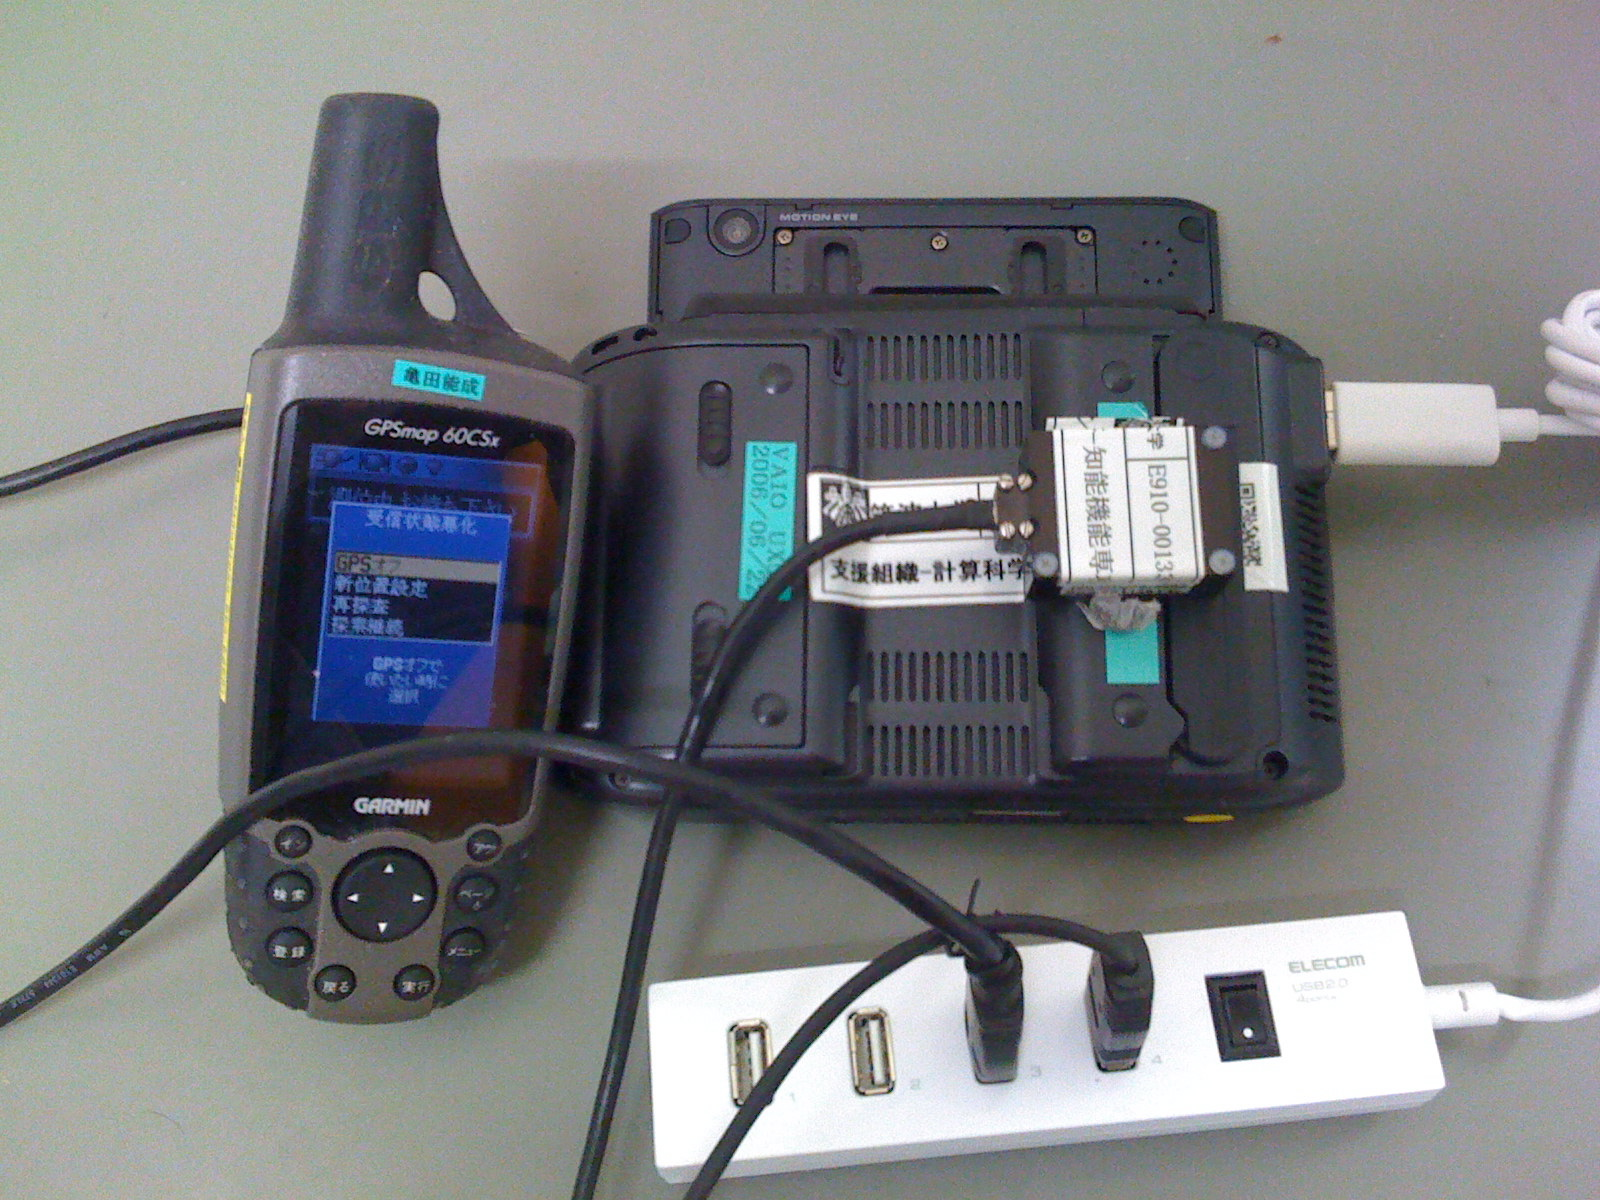
\includegraphics[width=14cm]{./Primitives/vaio_gps_gyro.jpg}
	\rule{35em}{0.5pt}
	\caption[Fusion of GPS and gyrocompass devices]{The Garmin GPSmap 60CSx (appendix \ref{AppendixGPS}) and InterSense InertiaCube3 (appendix \ref{AppendixGyro}) are connected to the Sony VAIO VGN-UX90PS via USB cable and hub}
	\label{fig:VAIOGPSGyro}
\end{figure}

The GSP and gyrocompass devices provide position and orientation information of the mobile device. Together with the prebuilt 3D scene model, we can render the visual aids to visualize viewing fields of surveillance cameras. The update rate of the gyrocompass is 180Hz, which is high thus the orientation information is quite good. However, the GPS device error is about 5--10 m (figure \ref{fig:GPSError}), which affects badly the accuracy of the visualization. To improve the GPS device error, model-based tracking method as described in \cite{Reference13} may be used.


\begin{figure}[htbp]
	\centering
	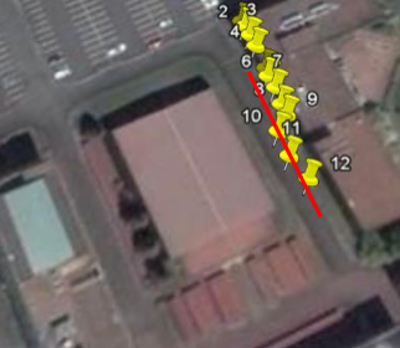
\includegraphics{./Primitives/gps_error.png}
	\rule{35em}{0.5pt}
	\caption[GPS error]{The points do not lie on the red line because of GPS error}
	\label{fig:GPSError}
\end{figure}

Although the more auxiliary devices we add the bulkier and more complicated in programming the mobile device becomes, GPS and gyrocompass devices can be used together with PTAM in the multi-sensor fusion \cite{Reference14} style, which may greatly improves the robustness of the system:

\begin{itemize}
	\item Initialization problem: the GPS and gyrocompass devices may provide initial position and orientation of the mobile device. Although the error of the GPS device is not small, in a large map it may help PTAM to reduce the search space.
	\item Quick movement: PTAM is image-based, thus it does not work well when the user quickly moves the mobile device. At this time, the gyrocompass may provide PTAM the orientation information because its update rate is high. Although the gyrocompass suffers from drifting error and needs to be continuously adjusted by the other sensors in the fusion, quick mobile device movement usually lasts only in a short time, thus gyrocompass may provide precious temporary information during this time.
\end{itemize}

%------------------------------------------------------------------------------

\section{Software Development Environment}

Visualization methods are expected to be found experimentally and visually. Thus, trial and error methodology is applied here. To shorten the trial and error cycle, we need a good development environment which allows quick compiling, running and modifying.

At first we used C/C++ language and OpenGL API \cite{Reference10}. Because both the language and the API are in too low level, the development speed was slow. Later, C/C++ language was fully replaced by Ruby language. Ruby is an object oriented strongly-typed dynamic language that attracts attention of developers world-wide in recent years. From the perspective of software engineering, the above features provide the following benefits:

\begin{itemize}
	\item Object oriented feature: Easy to structure the program and later maintain the source code over time.
	\item Strongly-typed feature: Variables have types, thus we can avoid bugs which usually occur in weakly-typed languages like PHP.
	\item Dynamic feature: There is no compile time. With static languages like C/C++, a lot time is wasted on compiling source code. With Ruby we can modify source code and run right away.
\end{itemize}

The development speed was better but still slow, partly because of the slow. It was concluded that the speed of the development is largely affected by the API rather than the language. Consequently, a higher level 3D rendering engine has been adopted: Irrlicht. Later, we read many reviews on the Internet that say that OGRE \cite{Reference11} is easier to use than Irrlicht, thus we migrated to OGRE. OGRE, Object-Oriented Graphics Rendering Engine, is a scene-oriented, flexible 3D rendering engine written in C++ designed to make it easier and more intuitive for developers to produce applications utilizing hardware-accelerated 3D graphics. The class library abstracts all the details of using the underlying system libraries like Direct3D and OpenGL and provides an interface based on world objects and other intuitive classes.

However, OGRE is generally used for creating 3D games thus contain too many features that we do not need. The framework forced us to write too much bloated code for the purpose of this research. As a result, we finally migrated to a combination of Ruby and C language with pure OpenGL API. At this time Ruby has grown to version 1.9. In this version the interpreter is replaced by a virtual machine, which boosts our Ruby program's speed to about 10x. Moreover importantly it is ridiculously easy to write C extension for Ruby \cite{Reference15}. For program parts that need speed like networking, video frame retrieving, and image processing, we use the Ruby standard library which is written in C, or write them as C extension for Ruby. For program parts that need trial-error or does not need speed like the user interface part, we write them in pure Ruby.

Programming for the iPhone requires Objective-C language, which is similar to C/C++ language. There are some difficulties programming for the iPhone, for example: the API to retrieve video frames from the iPhone camera is not documented, iPhone uses OpenGL ES 1.1 not the standard OpenGL. However, based on the program for the VAIO, we could create the program for the iPhone with some effort.

In short, our experience suggests that keeping a balance between dynamic language and static language is a good choice.
